%%%%%%%%%%%%%%%%%%%%%%%%%%%%%%%%%%%%%%%%%%%%%%%%%%%%%%%%%%%%%%%%%%%%%%%%%%%%%%%%%%%%%%%%%%%%%%%%%%%%%%%%%%
%%%   %%%%
%%%%%%%%%%%%%%%%%%%%%%%%%%%%%%%%%%%%%%%%%%%%%%%%%%%%%%%%%%%%%%%%%%%%%%%%%%%%%%%%%%%%%%%%%%%%%%%%%%%%%%%%%%%

\documentclass{sig-alternate}

\usepackage[utf8]{inputenc}
\usepackage{amssymb}
\setcounter{tocdepth}{3}
\usepackage{graphicx}
\usepackage{tabularx}
\usepackage{url}
\usepackage{listings}
\usepackage{subfigure}
\usepackage{algorithmic}
\usepackage{algorithm}


%\newcommand{\keywords}[1]{\par\addvspace\baselineskip
%\noindent\keywordname\enspace\ignorespaces#1}

% todo macro
\usepackage{color}
\newtheorem{deflda}{Axiom}
\newcommand{\todo}[1]{\noindent\textcolor{red}{{\bf \{TODO}: #1{\bf \}}}}
\newcommand{\neon}{NeOn }
\newcommand{\protege}{Prot{\'e}g{\'e} }



%%%%%%%%%%%%%%%%%%%%%%%%%%%%%%%
%%%  Beginning of document  %%%
%%%%%%%%%%%%%%%%%%%%%%%%%%%%%%%

\begin{document}

% first the title is needed
% --- ACM copyright metadata here ---
%\conferenceinfo{SEM}{14, September 04 - 05 2014, Leipzig, AA, Germany}
%\CopyrightYear{2015}
%\crdata{978-1-4503-2927-9/14/09.}


%\title{How to access and reuse ontologies in real-world scenarios}
\title{Practical Guidelines for reusing vocabularies in real-world scenarios: A LOV-based Approach}

\numberofauthors{3}
\author{
% 1st. author
\alignauthor Ghislain Auguste Atemezing\\
       \affaddr{MONDECA}\\
       \affaddr{35 boulevard Strasbourg, Paris, France}\\
       \email{\small{ghislain.atemezing@mondeca.com}}
% 3rd author
  \alignauthor Nuria Garc{\'i}a-Santa\\
       \affaddr{Expert System Iberia}\\
       \affaddr{Campo de las Naciones, Madrid, Spain.}\\
       \email{\small{ngarcia@expertsystem.com}}
% 2nd. author
\alignauthor Boris Villaz{\'o}n-Terrazas\\
       \affaddr{Expert System Iberia}\\
       \affaddr{Campo de las Naciones, Madrid, Spain.}\\
       \email{\small{bvillazon@expertsystem.com}}       
}

\maketitle


%%%%%%%%%%%%%%%%%%
%%%  Abstract  %%%
%%%%%%%%%%%%%%%%%%

\begin{abstract}
Developing ontologies, by reusing already available and well-known ontologies, is commonly acknowledge to play a crucial role to facilitate inclusion and expansion of the Web of Data. Some recommendations exist to guide ontologists in ontology engineering, but they do not provide guidelines on how to reuse vocabularies at low fine grained, i.e., reusing specific classes and properties. Moreover, it is still hard to find a tool that provides users with an environment to reuse terms. This paper presents Prot{\'e}g{\'e}LOV, a plugin for the ontology editor Prot{\'e}g{\'e}, that combines the access to the Linked Open Vocabularies (LOV) during ontology modeling. It allows users to search a term in LOV and provides three actions if the term exists : (i) replace the selected term in the current ontology; (ii) add the {\tt rdfs:subClassOf} or {\tt rdfs:subPropertyOf} axiom between the selected term and the local term; and (iii) add the {\tt owl:equivalentClass} or {\tt owl:equivalentProperty} between the selected term and local term. Results from a preliminary user study indicate that Prot{\'e}g{\'e}LOV does provide an intuitive access and reuse of terms in external vocabularies.
%\keywords{ontology engineering, ontology reuse, LOV, Prot{\'e}g{\'e}, Plugin} 
\end{abstract}

% Categories for the papers.
\todo{Find the right categories of the paper for acm}
\category{H.4}{Information Systems Applications}{Miscellaneous}
\category{H.3.5}{Online Information Services}{Data sharing}[Web-based services]

\terms{Accessibility, Linked Data, Vocabularies}

\keywords{ontology engineering, ontology reuse, LOV, Prot{\'e}g{\'e}, Plugin}



%%%%%%%%%%%%%%%%%%%%%%%%%
%%%  1. Introduction  %%%
%%%%%%%%%%%%%%%%%%%%%%%%%

%\vspace{-3mm}
\section{Introduction}\label{sec:introduction}
So far, Linked Data principles and practices are being adopted by an increasing number of data providers, getting as result a global data space on the Web containing hundreds of LOD datasets \cite{Heath_Bizer_2011}. There are already several guidelines for generating, publishing, interlinking, and consuming Linked Data \cite{Heath_Bizer_2011}. An important task, within the generation process, is to build the vocabulary to be used for modelling the domain of the data sources, and the common recommendation is to reuse as much as possible available vocabularies \cite{Heath_Bizer_2011,hyland14}. This reuse approach speeds up the vocabulary development, and therefore, publishers will save time, efforts, and resources. 

There are research efforts, like the NeOn Methodology \cite{suarezfigueroa2012ontology}, the Best Practices for Publishing Linked Data - W3C Working Group Note \cite{hyland14}, and the work proposed by Lonsdale et al. \cite{Lonsdale2010318}. However, at the time of writing we have not found specific and detailed guidelines that describe how to reuse available vocabularies at fine granularity level,i.e., reusing specific classes and properties. Our claim is that this difficulty in how to reuse vocabularies at low fine grained level is one of major barriers to the vocabulary development and in consequence to deployment of Linked Data.

Moreover, the recent success of Linked Open Vocabularies (LOV\footnote{\url{http://lov.okfn.org/dataset/lov/}}) as a central point for curated catalog of ontologies is helping to convey on best practices to publish vocabularies on the Web, as well as to help in the Data publication activity on the Web. LOV comes with many features, such as an API, a search function and a SPARQL endpoint.

In this paper we propose an initial set of guidelines for this task, and provide technological support by means of a plugin for \protege, which is one of the popular frameworks for developing ontologies in a variety of formats including OWL, RDF(S), and XML Schema. It is backed by a strong community of developers and users in many domains. One success on \protege also depends on the availability to extend the core framework adding new functionalities by means of plug-ins. In addition, we propose to explore, design and implement a plug-in of LOV in \protege for easing the development of ontologies by reusing existing vocabularies at low fine grained level. The tool helps to improve the modeling and reuse of ontologies used in the LOD cloud.

%, by providing the following features in Prot{\'e}g{\'e}:
%\begin{itemize}
%\item Import easily vocabularies from LOV into \protege. 
%\item Propose to the user a list of candidate vocabularies in LOV matching the term
%\item Have an updating mechanism (synchronization) to LOV catalog
%\item Check if a new vocabulary created in \protege satisfied the LOV recommendations \cite{pybernard12}
%\item Suggest to LOV a new created vocabulary within \protege.
%\end{itemize}

%This paper presents \protege, a first implementation of the LOV realized as a plugin for the ontology editor \protege. 
\vspace{-3mm}
\section{Reusing vocabulary elements when building ontologies}\label{sec:reuse}
In this section we describe the procedure of reusing available vocabulary terms when building ontologies. In a nutshell, the task of building vocabularies by reusing available vocabulary terms consists of
\vspace{-1mm}
\begin{itemize}
	\item Search for suitable vocabulary terms to reuse from the LOV repository. The search should be conducted by using the terms of the application domain.
	\item Assess the set of candidate terms from LOV repository. In this particular case the results coming from LOV repository include a score for each term retrieved.
	\item Select the most appropriate term taking into the account its score.
	\item Include the selected term in the ontology that has being developed. The selected term will be the external term. There are three alternatives in this case: 
	\begin{itemize}
		\item Include the external term and use it directly in the local ontology by defining local axioms to/from that term in the local ontology.
		\item Include the external term, create a local term, and define the {\tt rdfs:subClassOf} or {\tt rdfs:subPropertyOf} axiom to relate both terms.
		\item Include the external term, create a local term, and define the {\tt owl:equivalentClass} or {\tt owl:equivalentProperty} axiom to relate both terms. 				
	\end{itemize}
\end{itemize}





%%%%%%%%%%%%%%%%%%%%%%%%%%%%%%%%%%%%%%%%%%%%%%%%%%
%%%  2. Related work  %%%
%%%%%%%%%%%%%%%%%%%%%%%%%%%%%%%%%%%%%%%%%%%%%%%%%%
%\vspace{-3mm}
\section{Related Work}\label{sec:soa}
%\vspace{-3mm}
%Show here some work related to plugin for helping in ontology development:Neon and other
%\todo{target to guidelines}
%\todo{add more citation papers}
In the literature there exist many attempts to advise vocabulary publishers on the importance of reusing terms, as indicated in \cite{janowicz2014five,jimenez2008}. However, to the best of our knowledge there are not guidelines to help vocabulary practitioners to reuse vocabularies in real-world scenario, and considering specific ontology/vocabulary elements. 

In the W3C Government Linked Data best practice document \cite{hyland14}, reusing vocabularies is recommended by providing to stakeholders a basic checklist when using or extending a vocabulary. It gives general guidance to follow before publishing the vocabulary, not guidance during the creation of the vocabulary. Our proposal is to guide the users during the implementation process.

The BioPortal Reference Plugin\footnote{\url{http://protegewiki.stanford.edu/wiki/BioPortal_Reference_Plugin}} allows the user to insert into the ontology references to external ontologies and terminologies stored in BioPortal\footnote{\url{http://bioportal.bioontology.org/}}. The plugin allows to generate external reference of a selected term. Additionally, the BioPortal Import Plugin\footnote{\url{http://protegewiki.stanford.edu/wiki/BioPortal_Import_Plugin}} allows users to import classes from external ontologies stored in the BioPortal ontology repository. The user can import entire trees of classes with a desired depth and choose which properties to import for each class. However, those plugins work only with \protege 3.x releases and are not ported yet to recent versions. 

Most closely related to the {\protege}LOV plugin are approaches that use semantic search engine to support the process of editing an ontology and make large scale knowledge reuse automatically integrated in the tool. An example is the Watson Plugin \cite{neonguide2008} for the \neon Toolkit \cite{haase2008neon}, a plugin supporting the \neon life-cycle management using the Watson \cite{d2007watson} APIs\footnote{\url{http://watson.kmi.open.ac.uk/WS_and_API.html}}.However the similar plugin for Protege\footnote{\url{http://protegewiki.stanford.edu/wiki/Watson_Search_Preview}} is just a proof of concept rather than a real plugin.

 


\section{Reusing vocabulary terms\\ when building ontologies}\label{sec:reuse}
\todo{We have to improve this section- add a picture for workflow}
\todo{Boris will do it}

In this section, we describe the workflow for reusing available vocabulary terms when building ontologies based on an existing catalogue of vocabularies. Recall that we do not specify which the expressivity of the resulting ontology. We foresee that the resulting ontology is likely to be a lightweight ontology. However the data publisher is responsible for adding more semantics when reusing existing vocabulary terms. Figure \ref{} depicts the proposed workflow. 

\subsection{Use case scenario: lobid vocabulary}
\label{lobid vocabulary}
Looking at the evolution of some vocabularies with highest changes since their release in LOV,\texttt{lobid} vocabulary is the winner with 16 modifications. The \texttt{lobid} vocabulary\footnote{\url{http://purl.org/lobid/lv}} is a vocabulary designed for the  linking open bibliographic data services. The ontology was first published on 2012-03-02 with only two properties, a minimal metadata information and labels in English. Since then, there have been 15 different versions and the current version (version of 2015-02-09) of the ontology contains 8 classes and 16 properties. Based on the different changes occurred during the on-going development of the lobid vocabulary, vocabulary changes can be grouped in two categories:
\begin{itemize}
\item Editorial changes (EDc) are the ones related with labels and comments translations, typos fixed. Those changes don't affect the structure of the vocabulary.
\item Semantic changes (SMc) are related with modifying the structure of the vocabulary, by either adding new axioms, new classes and properties.
\end{itemize}

Furthermore, the semantic changes can be broken down in four categories related to the main parts of a vocabulary, that are metadata, classes, properties and axioms. Thus we can group them as follows:

\begin{itemize}
\item Metadata changes (MTc), when the changes are related with the metadata section of the vocabulary. E.g., adding provenance information, license, publishers and creators data.
\item Property changes (PPc), when updating the vocabulary 
\item Classes changes (CLc), such as the creation of named classes.
\item Axioms changes (AXc) for updates using some axioms for restrictions in or the creation of anonymous classes. 

\end{itemize}

Table \ref{tab:lobid} summarizes the number of changes for the lobid vocabulary. In  a total of 20 changes, only 2 are editorial changes and each time accompanied with a semantic change in the corresponding version.
\texttt{lobid} vocabulary is a good example of reusing existing terms where the definition of all the classes are ``subclassing'' of three existing vocabularies: \texttt{dct}, \texttt{bibo} and \texttt{archives}\footnote{\url{http://data.archiveshub.ac.uk/def/}}.  

\begin{table}[!htb]
\centering{

\begin{tabular}{lccccc}
\hline
 \textbf{Changes} & EDc & MTc & PPc & CLc & AXc \\ \hline
  Numbers & 2 & 4 & 8 & 3 & 3 \\
 
 \hline
\end{tabular}
\caption{Changes observed in the lobid vocabulary since its release in 2012. }
\label{tab:lobid}
}
\end{table}

\subsection{Workflow on Reusing Terms}
In a nutshell, the task of building vocabularies by reusing available vocabulary terms consists of the following steps:

\begin{itemize}
	\item Searching for suitable vocabulary terms to reuse from the any vocabulary repository, such as BioPortal, LOV, Bartoc.org\footnote{\url{http://bartoc.org}}, etc. The search should be conducted by using the terms of the application domain.
	\item Assessing the set of candidate terms from the vocabulary repository. In the particular case of LOV, the results include a score related to their ``importance'' in the corpus for each term retrieved.
	\item Selecting the most appropriate term taking into the account its score from the candidates terms proposed. Other criteria can be also considered here: (i) the stability of the URI namespace, (ii) the trustworthiness of the publisher of the vocabulary and (iii) the presence or absence of a community using the vocabulary.
	\item Including the selected term in the ontology that has being developed. The selected term will be the external term. There are three alternatives in this case: 
	\begin{itemize}
		\item Include the external term and use it directly in the local ontology by defining local axioms to or from that term in the local ontology.
		\item Include the external term, create a local term, and define the {\tt rdfs:subClassOf} or {\tt rdfs:subPropertyOf} axiom to relate both terms.
		\item Include the external term, create a local term, and define the {\tt owl:equivalentClass} or \\ {\tt owl:equivalentProperty} axiom to relate both terms. 				
	\end{itemize}
\end{itemize}



%%%%%%%%%%%%%%%%%%%%%%%%%%%%%%%%%%%%%%%%%%%%%%%%%%%
%%%  3.LOV APIs Description  %%%
%%%%%%%%%%%%%%%%%%%%%%%%%%%%%%%%%%%%%%%%%%%%%%%%%%%
%\vspace{-3mm}
%\section{Linked Open Vocabulaires (LOV)}\label{sec:lov}
\section{Technological Support}
%\vspace{-3mm}
Include the technological support
\begin{itemize}
	\item protege
	\item lov
	\item protege LOV plugin
\end{itemize}


The intended purpose of the LOV \cite{vandenbusschelov} is to help users to find and reuse terms of vocabularies in Linked Open Data. For achieving that purpose, the LOV gives access to vocabularies metadata and terms using programmatic access with APIs.  
LOV\footnote{\url{http://lov.okfn.org/dataset/lov/}} catalogue is a hub of curated vocabularies used in the Linked Open Data Cloud, as well as other vocabularies suggested by users for their reuse. 
Some of the three main features of the LOV are for: (1) searching ontologies according to their scope, (2) assessing ontologies by providing a score for each term retrieved by a keyword search and (3) interconnecting ontologies using VOAF vocabulary\footnote{\url{http://lov.okfn.org/vocab/voaf}}.
The search function uses an algorithm based on the term
popularity in LOD and in the LOV ecosystem. The matched resource set for each term should be the value of the a) {\tt rdfs:label} b) {\tt rdfs:comment}, or c) {\tt rdfs:description} property.

%\begin{enumerate}
%\item Searching ontologies: It is the main LOV's feature is the search of vocabulary terms. These vocabularies are categorized within LOV according to the domain they address. In this way, LOV contributes to ontology search by means of (a) keyword search and (b) domain browsing.
% \item Assessing ontologies: LOV provides a score for each term retrieved by a keyword search. This score can be used during the assessment stage.
% \item Interconnecting ontologies: In LOV, vocabularies rely on each other in seven different ways. These relationships are explicitly stated using VOAF vocabulary\footnote{\url{http://lov.okfn.org/vocab/voaf}}. 
%\end{enumerate}

Futhermore, the LOV APIs give a remote access to the many functions of LOV through a set of RESTful services\footnote{\url{http://lov.okfn.org/dataset/lov/apidoc/}}. %The basic design requirements for these APIs is that they should allow applications to get access to the very same information humans do via the User Interfaces. More precisely the
The APIs give access through three different type of services related to: (1) vocabulary terms (classes, properties, datatypes and instances), (2) vocabulary browsing and (3) ontology's creators. 

%\begin{enumerate} 
%	\item vocabulary terms (classes, properties, datatypes and instances) providing functions to query the LOV search engine, with autocompletion features;
%	\item vocabulary browsing, in which a client can get access to the current list of vocabularies contained in the LOV catalogue and search for vocabularies for further purpose;
%	\item agents, or the ontology's creators, contributors or organizations. It also contains the search with autocompletion of an agent.
%	\end{enumerate}

%to continue 





%%%%%%%%%%%%%%%%%%%%%%%%%%%%%%%%%%%%%%%%%%%%%%%%%%%
%%%  4.ProtegeLOV Description  %%%
%%%%%%%%%%%%%%%%%%%%%%%%%%%%%%%%%%%%%%%%%%%%%%%%%%%
%\vspace{-3mm}
%\section{Prot{\'e}g{\'e}LOV}\label{sec:classification}
%Prot{\'e}g{\'e}LOV is an open source tool that provides support to the methodological guidelines described in section \ref{sec:reuse}. It is written in Java programming language as a plugin for the \protege ontology editor. It can be easily installed by just copying the jar file provided at the Prot{\'e}g{\'e}LOV website\footnote{\url{http://labs.mondeca.com/protolov/}} into the plugins directory of an existing \protege installation. Then upon a new start, the user should select \emph{Linked Open Vocabularies} item, within the \emph{Ontology views} menu item.

Currently, Prot{\'e}g{\'e}LOV\footnote{A video is also available at \url{https://www.youtube.com/watch?v=UgA17N5FNzA}} provides the following five functionalities: 

\begin{enumerate}
\vspace{-1mm}\item \textbf{Search for a particular term (class or property) in LOV repository}. 
The user selects a particular term from the \emph{Class}, \emph{Object property} or \emph{Data property} navigator. 
Next, the user switches to the \emph{Linked Open Vocabularies View} and performs a search on the LOV repository. The system takes as input the selected term, and calls the LOV REST API to get the LOV terms that match the criteria.
The plugin provides the following information (if it is available) for each term (1) URI, (2) score, (3) label, (4) local name, and (5) usage note.

%\vspace{-1mm}\item \textbf{Browse the list of terms, from LOV repository, which matches the search criteria}. The system takes as input the selected term, and calls the LOV REST API to get the LOV terms that match the criteria.
%The plugin provides the following information (if it is available) for each term (1) URI, (2) score, (3) label, (4) local name, and (5) usage note.

\vspace{-1mm}\item \textbf{Reuse directly a particular term from LOV repository}
The user selects the \emph{reuse directly} option. Next, the system replaces the selected term from the \emph{Class}, \emph{Object property} or \emph{Data property} navigator, and replaces by the selected term from LOV.

\vspace{-1mm}\item \textbf{Add the particular term and define the {\tt owl:equivalentClass} or {\tt owl:equivalentProperty} axiom}.
The user selects the \emph{add entity and equivalent axiom} option. Next, the system includes the new term on the local ontology, and defines {\tt owl:equivalentClass} or {\tt owl:equivalentProperty} axiom to relate both terms.

\vspace{-1mm}\item \textbf{Add the particular term and define the {\tt rdf:subClassOf} or {\tt rdfs:sub-}\\
{\tt PropertyOf} axiom}. The user selects the \emph{add entity and sub-entity axiom} option. Next, the system includes the new term on the local ontology, and defines {\tt rdfs:subClassOf} or {\tt rdfs:subPropertyOf} axiom to related both terms.
\end{enumerate}

Figure \ref{fig:LOVoptions} depicts the three main actions the user can perform. % on the selected LOV term. 

\begin{figure}[b!ht]
\center
\includegraphics[scale=0.4]{img/LOVOptions.png}
\caption{Three actions currently available in the plugin after looking up a term in LOV catalogue: (a) reuse it directly, (b) add equivalent axiom and (c) add subEntity axiom}
\label{fig:LOVoptions}
\end{figure}


%\begin{figure}[!bht]
%\center
%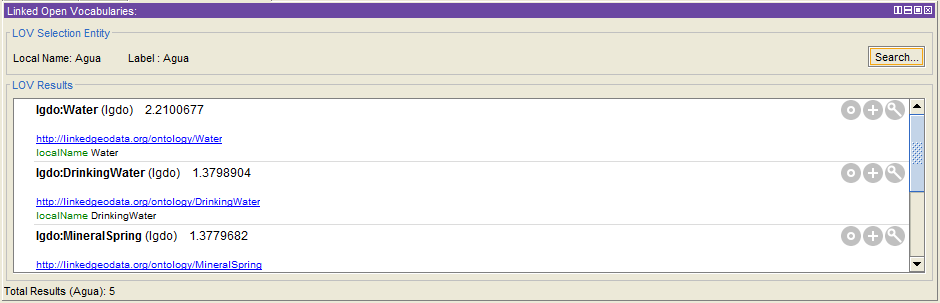
\includegraphics[scale=0.5]{img/LOVmockup.png}
%\label{fig:LOVresults}
%\caption{Panel showing the results for searching a term in the class hierarchy.}
%\end{figure}



%%%%%%%%%%%%%%%%%%%%%%%%%%%%%%%%%%%%%%%
%%%  5. Conclusion and Future Work  %%%
%%%%%%%%%%%%%%%%%%%%%%%%%%%%%%%%%%%%%%%
%\vspace{-3mm}
\section{Evaluation}\label{sec:conclusion}
We have conducted an initial user driven evaluation of the tool. For this preliminary evaluation we keep the number of evaluators low; seven ontology engineers used our plugin and gave us an insight on their experience by filling in a questionnaire \footnote{\url{http://goo.gl/H4YgBJ}}. The results indicate that while the tool needs some minor improvements, the majority of the evaluators still consider the tool to be useful.

\vspace{-3mm}
\section{Conclusions and Future Work}\label{sec:conclusions}
In this paper we have presented (1) initial guidelines that describe how to reuse available vocabularies at low fine grained level,i.e., reusing specific classes and properties, and (2) a tool that provides technological support by means of a plugin for \protege that access LOV API. As future work we plan to fully evaluate the tool and guidelines.






%%%%%%%%%%%%%%%%%%%%%%%%%
%%%  Acknowledgments  %%%
%%%%%%%%%%%%%%%%%%%%%%%%%
%\vspace{-1mm}
\paragraph{\textbf{Acknowledgments.}} %\label{sec:acknowledgments}
Thanks to Pierre-Yves and the LOV team for maintaining the LOV catalog and the API access.
% More acknowledgments here
%\vspace{-3mm}

\bibliographystyle{abbrv}
%\nocite{*}
\bibliography{isemanticsbib}
\balancecolumns
\end{document}
